\section{Séance 4 : Offre de travail et de capital}


\subsection{Offre de travail}



\begin{tabular}{lll}
	Heures de travail & $\Rightarrow$ & $Tr$\\
	Heures de loisir  & $\Rightarrow$ & $Loi$\\
	Salaire horaire   & $\Rightarrow$ & $Wh$\\
	Revenu journalier & $\Rightarrow$ & $Y$\\
\end{tabular}

$$1\ journee = 24\ heures = Tr + Loi$$
$$Y = Wh * Tr$$



\subsubsection{Substitut et complément}



Si la consommation de biens est un \textbf{substitut} aux loisirs :
\begin{itemize}
	\item une \textbf{hausse} de Wh entraîne toujours une \textbf{augmentation} de Tr et de Y à l'optimum ;
	\item une \textbf{baisse} de Wh entraîne toujours une \textbf{diminution} de Tr et de Y à l'optimum.
\end{itemize}
Il aime travailler, il est motivé à travailler plus pour gagner plus.


\vspace{0.5cm}


Si la consommation de biens est un \textbf{complément} aux loisirs :
\begin{itemize}
	\item une \textbf{hausse} de Wh ne change pas Tr mais augmente Y à l'optimum ;
	\item une \textbf{baisse} de Wh ne change pas Tr mais augmente Y à l'optimum.
\end{itemize}
Il n'aime pas travailler, il ne travaille pas plus si il gagne plus.\\


\subsubsection{Graphiques}



\begin{center}
	\begin{tabular}{cc}
		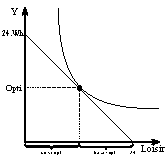
\includegraphics[width=0.25\textwidth]{images/graph_offre_de_travail.pdf} & 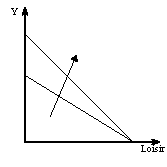
\includegraphics[width=0.25\textwidth]{images/graph_offre_de_travail_wh_augmente.pdf}\\
		Complet                                                                   & Si $Wh$ augmente
	\end{tabular}
\end{center}


\newpage
\subsection{Offre de capital}



\begin{tabular}{lll}
	Consommation en 1ère période  & $\Rightarrow$ & $C_t$\\
	Consommation en 2ème période  & $\Rightarrow$ & $C_{t+1}$\\
	Revenu en 1ère période        & $\Rightarrow$ & $Y_t$\\
	Revenu en 2ee période         & $\Rightarrow$ & $Y_{t+2}$\\
	Épargne                       & $\Rightarrow$ & $S_t$\\
	Taux d'intérêt                & $\Rightarrow$ & $r$\\
	Cherche à maximiser l'utilité & $\Rightarrow$ & $U(C_t,C_{t+1})$
\end{tabular}
$$S_t = Y_t - C_t$$
\begin{flushright}
	(si St < 0 : emprunt)
\end{flushright}
$$C_{t+1} = Y_{t+1} + ( 1 + r ) * S_t $$



\subsubsection{Graphiques}



\begin{center}
	\begin{tabular}{ccc}
		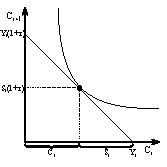
\includegraphics[width=0.25\textwidth]{images/graph_offre_de_capital_ytplus1_nulle.pdf} & 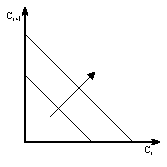
\includegraphics[width=0.25\textwidth]{images/graph_offre_de_capital_ytplus1_nulle_yt_augmente.pdf} & 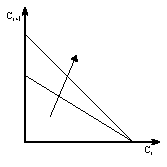
\includegraphics[width=0.25\textwidth]{images/graph_offre_de_capital_ytplus1_nulle_r_augmente.pdf}\\
		Cas où $Y_t>0$ et $Y_{t+1}=0$             &             Si $Y_t$ augmente             &             Si $r$ augmente
	\end{tabular}
\end{center}